\chapter{Floating Point}
\label{c-fp}


The main goal of this chapter is to introduce floating point numbers and the issues around their use and misuse.  Toward that end, we will first cover fixed point numbers.


\section{Fixed Point Numbers}


\vspace{.1in}\noindent
\textbf{Example:}


Convert $\pi$ to binary and hexadecimal.  Assume you have four
bits before the radix point and 8 bits after the radix point.

Sol:

before the decimal we have $3=0011$

after the decimal

\begin{tabular}{l|l}
$0.1415926\ldots$ & \\
\hline
$0.2831852$ & 0 \\
$0.5663704$ & 0 \\
$1.1327408$ & 1 \\
$0.2654816$ & 0 \\
$0.5309632$ & 0 \\
$1.0619264$ & 1 \\
$0.1238528$ & 0 \\
$0.2477056$ & 0 \\
\end{tabular}

combining gives $0011.00100100$

To convert to hexadecimal we group the digits together in groups of four starting at the radix point, thus we are forcing the hexadecimal digits to represent either integer or fractional portions.

\begin{tabular}{|c|c|c|}\hline
0011 & 0010 & 0100 \\ \hline
3    & 2    & 4    \\ \hline
\end{tabular}

Thus the answer is $0x3.24$.




\vspace{.1in}\noindent
\textbf{Example:}


Convert 25.6875 to binary.

    {\color{ans}
    \begin{tabular}{r|lcr|l}
    25 & /2 &.& *2 & .6875 \\ \hline
    12 & 1  & &  1 & .375  \\
     6 & 0  & &  0 & .75   \\
     3 & 0  & &  1 & .5    \\
     1 & 1  & &  1 & 0     \\
     0 & 1  & &    &
     \end{tabular}

     11001.1011
    }


\section{Floating Point Numbers}

I came up with the following program in my doctoral work at UCSB.

\begin{verbatim}
#include <iostream>
#include <iomanip>
#include <cmath>

using namespace std;

int main(){
    double pi, e, result;
    int i;

    e=exp(1);

    pi=atan(1)*4;

    result=pi;

    for(i=1;i<53;i++){
        result=sqrt(result);
    }

    for(i=1;i<53;i++){
        result=result*result;
    }

    cout << setiosflags(ios::showpoint | ios::fixed) << setprecision(16);
    cout << "Pi     = " << pi << endl;
    cout << "Result = " << result << endl;
    cout << "e      = " << e << endl;

    return 0;
}
\end{verbatim}

The results are

\begin{verbatim}
Pi     = 3.1415926535897931
Result = 2.7182818081824731
e      = 2.7182818284590451
Press any key to continue
\end{verbatim}

Notice that Result is $e$ to 7 significant digits, but it should be $\pi$.  This underscores the importance of being numerically aware when writing programs.


\section{IEEE 754}

Floating point numbers are based off scientific notation.  Consider a typical number in base 10 scientific notation,
\begin{eqnarray*}
  -1.23 \times 10^{3}.
\end{eqnarray*}
The number is composed of five pieces of information,
\begin{enumerate}
    \item sign of the number (-),
    \item significant or mantissa (1.23),
    \item base (10),
    \item sign of the exponent (+),
    \item magnitude of the exponent (3).
\end{enumerate}


There are two basic number formats called out in IEEE 754, single precision (float in c/c++), and double precision (double in c/c++).  In addition there are two extended formats, which are only used as intermediate results while calculating.
\vspace{6pt}

\begin{tabular}{|c|c|c|c|}
  \hline
   e & f & Category & Interpretation \\
  \hline
    & $1\ldots 11$ & &  \\
   $1\ldots 11$ & $\vdots$ & NaN & See Codes \\
    & $0\ldots 01$ & &  \\ \hline
   $1\ldots 11$ & $0\ldots 00$ & $\pm\infty$ & $\pm\infty$ \\ \hline
   $1\ldots 10$ & $1\ldots 11$ & &  \\
   $\vdots$ & $\vdots$ & Numbers & $(-1)^s\times 1.f \times 2^{(e-127)}$ \\
   $0\ldots 01$ & $0\ldots 00$ & &  \\ \hline
    & $1\ldots 11$ & &  \\
   $0\ldots 00$ & $\vdots$ & Denormals & $(-1)^s\times 0.f \times 2^{(-126)}$ \\
    & $0\ldots 00$ & &  \\ \hline
   $0\ldots 00$ & $0\ldots 00$ & $\pm 0$ & $\pm 0$ \\ \hline
\end{tabular}

\vspace{6pt}\noindent
NaN codes:
\vspace{6pt}

\begin{tabular}{|c|c|c|}
  \hline
  Dec & Meaning                & Example \\ \hline
  1   & invalid square root    & $\sqrt{-1}$ \\
  2   & invalid addition       & $\infty + -\infty$ \\
  4   & invalid division       & $\frac{0}{0}$ \\
  8   & invalid multiplication & $0\times\infty$ \\
  9   & invalid modulo         & $x mod 0$ \\
   \hline
\end{tabular}

For this discussion, the notation $fl(x)$ will be used to mean the number $x$ as it is represented in floating point on a computer.


$$
(-1)^s\cdot 1.f\times 2^{e-127}
$$

\noindent
\begin{tabular}{c@{\extracolsep{5pt}}c@{}c@{}c@{}c@{}c@{}c@{}c@{}c@{}c@{}c@{}c@{}c@{}c@{}c@{}c@{}c@{}c@{}c@{}c@{}c@{}c@{}c@{}c@{}c@{}c@{}c@{}c@{}c@{}c@{}c@{}c}
  0 & 0 & 0 & 0 & 0 & 0 & 0 & 0 & 0 & 1 & 1 & 1 & 1 & 1 & 1 & 1 & 1 & 1 & 1 & 2 & 2 & 2 & 2 & 2 & 2 & 2 & 2 & 2 & 2 & 3 & 3 & 3 \\
  1 & 2 & 3 & 4 & 5 & 6 & 7 & 8 & 9 & 0 & 1 & 2 & 3 & 4 & 5 & 6 & 7 & 8 & 9 & 0 & 1 & 2 & 3 & 4 & 5 & 6 & 7 & 8 & 9 & 0 & 1 & 2 \\
  \hline
  \multicolumn{1}{|c}{s} & \multicolumn{8}{|c}{e} & \multicolumn{23}{|c|}{f} \\
  \hline
\end{tabular}


This is equivalent to saying


$$
(-1)^s\cdot 1.f\times 2^E
$$

\noindent
\begin{tabular}{c@{\extracolsep{5pt}}c@{}c@{}c@{}c@{}c@{}c@{}c@{}c@{}c@{}c@{}c@{}c@{}c@{}c@{}c@{}c@{}c@{}c@{}c@{}c@{}c@{}c@{}c@{}c@{}c@{}c@{}c@{}c@{}c@{}c@{}c}
  0 & 0 & 0 & 0 & 0 & 0 & 0 & 0 & 0 & 1 & 1 & 1 & 1 & 1 & 1 & 1 & 1 & 1 & 1 & 2 & 2 & 2 & 2 & 2 & 2 & 2 & 2 & 2 & 2 & 3 & 3 & 3 \\
  1 & 2 & 3 & 4 & 5 & 6 & 7 & 8 & 9 & 0 & 1 & 2 & 3 & 4 & 5 & 6 & 7 & 8 & 9 & 0 & 1 & 2 & 3 & 4 & 5 & 6 & 7 & 8 & 9 & 0 & 1 & 2 \\
  \hline
  \multicolumn{1}{|c}{s} & \multicolumn{8}{|c}{e=E+127} & \multicolumn{23}{|c|}{f} \\
  \hline
\end{tabular}

They are the same because $e-127=E$ is the same equation as $e=E+127$.  I think the latter is easier to use because you read $E$ from the number and want $e$.  The first form (standard for most texts) involves you guessing what number produced what you are seeing (rather than calculating it).  It is like trying to solve $y=mx+b$ for $y$ given $x$ but using the form $\frac{(y-b)}{m}=x$ to do it.  It works, just not well.  In any case, consider some examples.

\vspace{.1in}\noindent
\textbf{Example:}

Convert $7.892$ to single precision IEEE.

\noindent
Step 1: Convert 7.892 to binary

$7.892 = 111.1110010001011010000111$

%0.892
%1.784
%1.568
%1.136
%0.272
%0.544
%1.088
%0.176
%0.352
%0.704
%1.408
%0.816
%1.632
%1.264
%0.528
%1.056
%0.112
%0.224
%0.448
%0.896
%1.792
%1.584
%1.168

\noindent
Step 2: Normalize and note sign

$7.892 =(-1)^0 1.111110010001011010000111\times 2^2$

\noindent
Step 3: Calculate Excess 127 code for exponent

$e=2+127=129=10000001$

\noindent
Step 4:Round $1.f$ to 24 digits

$fl(1.111110010001011010000111)=1.11111001000101101000100$

\noindent
Step 5: Assemble


\begin{tabular}{|c@{ }|c@{\extracolsep{5pt}}c@{}c@{}c@{}c@{}c@{}c@{}c@{ \extracolsep{0pt}}|c@{\extracolsep{5pt}}c@{}c@{}c@{}c@{}c@{}c@{}c@{}c@{}c@{}c@{}c@{}c@{}c@{}c@{}c@{}c@{}c@{}c@{}c@{}c@{}c@{}c|}
\hline
0 & 1 & 0 & 0 & 0 & 0 & 0 & 0 & 1 & 1 & 1 & 1 & 1 & 1 & 0 & 0 & 1 & 0 & 0 & 0 & 1 & 0 & 1 & 1 & 0 & 1 & 0 & 0 & 0 & 1 & 0 & 0 \\
  \hline
\end{tabular}






\vspace{.1in}\noindent
\textbf{Example:}


Calculate $3.75\times 29.625$ in IEEE-754 single precision floating point.

    {\color{ans}
    Convert:

    $3.75=11.11=1.111\times 2^1$

    $29.625=11101.101=1.1101101\times 2^4$

    \vspace{12pt}
    Multiply Significants:

    \vspace{6pt}
    \begin{tabular}{cccccccccccc}
     &1.&1&1&0&1&1&0&1& & &  \\
$\times$&1.&1&1&1& & & & & & &  \\ \hline
     &1.&1&1&0&1&1&0&1& & &  \\
     &0.&1&1&1&0&1&1&0&1& &  \\
     &0.&0&1&1&1&0&1&1&0&1&  \\
     &0.&0&0&1&1&1&0&1&1&0&1 \\ \hline
    1&1.&0&1&1&1&1&0&0&0&1&1
    \end{tabular}

    $1.10111100011\times 2^1$

    \vspace{12pt}
    Add exponents to normalization exponent and put in excess 127:

    \vspace{6pt}
    $1+4+1+127=133=10000101$

    \vspace{12pt}
    Write in single precision:

    \vspace{6pt}
    \begin{tabular}{|c|c|c|}\hline 0 & 10000101 & 1011 1100 0110 0000 0000 000 \\ \hline \end{tabular}


    }






\vspace{.1in}\noindent
\textbf{Example:}

Perform the following for IEEE-754, single precision
    \begin{enumerate}
        \item Show the representation of $x=93.3125$

        {\color{ans}

        $x=93.125_{10}=1011101.001_2=1.011101001\times 2^6$

\noindent
\begin{tabular}{|c@{\extracolsep{0pt} }|c@{\extracolsep{5pt}}c@{}c@{}c@{}c@{}c@{}c@{}c@{\extracolsep{0pt} }|c@{\extracolsep{5pt}}c@{}c@{}c@{}c@{}c@{}c@{}c@{}c@{}c@{}c@{}c@{}c@{}c@{}c@{}c@{}c@{}c@{}c@{}c@{}c@{}c@{}c|}
\hline                            %
0 & 1 & 0 & 0 & 0 & 0 & 1 & 0 & 1 & 0 & 1 & 1 & 1 & 0 & 1 & 0 & 0 & 1 & 0 & 0 & 0 & 0 & 0 & 0 & 0 & 0 & 0 & 0 & 0 & 0 & 0 & 0 \\
  \hline
\end{tabular}
        }

        \item calculate $x*y$ for $y$ equal to

\noindent
\begin{tabular}{|c@{\extracolsep{0pt} }|c@{\extracolsep{5pt}}c@{}c@{}c@{}c@{}c@{}c@{}c@{\extracolsep{0pt} }|c@{\extracolsep{5pt}}c@{}c@{}c@{}c@{}c@{}c@{}c@{}c@{}c@{}c@{}c@{}c@{}c@{}c@{}c@{}c@{}c@{}c@{}c@{}c@{}c@{}c|}
\hline                            %
0 & 1 & 0 & 0 & 0 & 0 & 0 & 0 & 0 & 0 & 0 & 0 & 0 & 0 & 0 & 0 & 0 & 0 & 0 & 0 & 0 & 0 & 0 & 0 & 0 & 0 & 0 & 0 & 0 & 1 & 0 & 0 \\
  \hline
\end{tabular}

    {\color{ans}
    exponent: 128+133-127=134

    float: shortcut, note that $y$ only has two 1's in the expansion (hidden and near end) and they are farther apart than the length of the significant portion of $x$.  This will cause the $x$ float to be placed starting at these locations.  The comma below notes where the last bit of precision lies.
\begin{eqnarray*}
z_{fl} & = & 1.01110100100000000000101,1101001
\end{eqnarray*}
Note that the first bit after the comma is a 1 so the number gets rounded up.

        z is

\noindent
\begin{tabular}{|c@{\extracolsep{0pt} }|c@{\extracolsep{5pt}}c@{}c@{}c@{}c@{}c@{}c@{}c@{\extracolsep{0pt} }|c@{\extracolsep{5pt}}c@{}c@{}c@{}c@{}c@{}c@{}c@{}c@{}c@{}c@{}c@{}c@{}c@{}c@{}c@{}c@{}c@{}c@{}c@{}c@{}c@{}c|}
\hline                            %
0 & 1 & 0 & 0 & 0 & 0 & 1 & 1 & 0 & 0 & 1 & 1 & 1 & 0 & 1 & 0 & 0 & 1 & 0 & 0 & 0 & 0 & 0 & 0 & 0 & 0 & 0 & 0 & 0 & 1 & 1 & 0 \\
  \hline
\end{tabular}
    }

    \end{enumerate}



\vspace{.1in}\noindent
\textbf{Example:}

Convert 3.03125 to IEEE single precision

    {\color{ans}
    \begin{tabular}{c|ccc|c}
      3 &   & . &   & 03125 \\ \hline
      1 & 1 &   & 0 & 0625  \\
      0 & 1 &   & 0 & 125  \\
        &   &   & 0 & 25  \\
        &   &   & 0 & 5  \\
        &   &   & 1 & 0  \\
    \end{tabular}

    $3.03125_{10}=11.00001_2=1.100001_2\times 2^1$

    $1+127 = 128$

    \begin{tabular}{|c@{ }|c@{\extracolsep{5pt}}c@{}c@{}c@{}c@{}c@{}c@{}c@{ \extracolsep{0pt}}|c@{\extracolsep{5pt}}c@{}c@{}c@{}c@{}c@{}c@{}c@{}c@{}c@{}c@{}c@{}c@{}c@{}c@{}c@{}c@{}c@{}c@{}c@{}c@{}c@{}c|}
\hline
0 & 1 & 0 & 0 & 0 & 0 & 0 & 0 & 0 & 1 & 0 & 0 & 0 & 0 & 1 & 0 & 0 & 0 & 0 & 0 & 0 & 0 & 0 & 0 & 0 & 0 & 0 & 0 & 0 & 0 & 0 & 0 \\
  \hline
\end{tabular}
    }

Now perform the following on your result and

\begin{tabular}{|c@{ }|c@{\extracolsep{5pt}}c@{}c@{}c@{}c@{}c@{}c@{}c@{ \extracolsep{0pt}}|c@{\extracolsep{5pt}}c@{}c@{}c@{}c@{}c@{}c@{}c@{}c@{}c@{}c@{}c@{}c@{}c@{}c@{}c@{}c@{}c@{}c@{}c@{}c@{}c@{}c|}
\hline
0 & 1 & 0 & 0 & 0 & 0 & 1 & 0 & 0 & 0 & 0 & 0 & 0 & 0 & 0 & 0 & 1 & 0 & 0 & 0 & 0 & 0 & 0 & 0 & 1 & 0 & 0 & 0 & 0 & 0 & 0 & 0 \\
  \hline
\end{tabular}
\begin{enumerate}
    \item Addition

    {\color{ans}
    $x=1.0000000100000001_2\times 2^5$

    $y=1.100001_2\times 2^1=0.0001100001_2\times 2^5$

    \begin{eqnarray*}
    x+y & = & 1.0000000100000001_2\times 2^5+0.0001100001_2\times 2^5 \\
        & = & (1.0000000100000001_2+0.0001100001_2)\times 2^5 \\
        & = & (1.0001100101000001_2)\times 2^5
    \end{eqnarray*}

\begin{tabular}{|c@{ }|c@{\extracolsep{5pt}}c@{}c@{}c@{}c@{}c@{}c@{}c@{ \extracolsep{0pt}}|c@{\extracolsep{5pt}}c@{}c@{}c@{}c@{}c@{}c@{}c@{}c@{}c@{}c@{}c@{}c@{}c@{}c@{}c@{}c@{}c@{}c@{}c@{}c@{}c@{}c|}
\hline
0 & 1 & 0 & 0 & 0 & 0 & 1 & 0 & 0 & 0 & 0 & 0 & 1 & 1 & 0 & 0 & 1 & 0 & 1 & 0 & 0 & 0 & 0 & 0 & 1 & 0 & 0 & 0 & 0 & 0 & 0 & 0 \\
  \hline
\end{tabular}
    }

    \item Multiplication
    {\color{ans}

    exponent is $132+128-127=133$

    significant is $1.0000000100000001\times 1.100001 = 1.1000010110000101100001$

\begin{tabular}{|c@{ }|c@{\extracolsep{5pt}}c@{}c@{}c@{}c@{}c@{}c@{}c@{ \extracolsep{0pt}}|c@{\extracolsep{5pt}}c@{}c@{}c@{}c@{}c@{}c@{}c@{}c@{}c@{}c@{}c@{}c@{}c@{}c@{}c@{}c@{}c@{}c@{}c@{}c@{}c@{}c|}
\hline
0 & 1 & 0 & 0 & 0 & 0 & 1 & 0 & 1 & 1 & 0 & 0 & 0 & 0 & 1 & 0 & 1 & 1 & 0 & 0 & 0 & 0 & 1 & 0 & 1 & 1 & 0 & 0 & 0 & 0 & 1 & 0 \\
  \hline
\end{tabular}
    }

\end{enumerate}






\vspace{.1in}\noindent
\textbf{Example:}

Perform the following for IEEE-754, single precision
    \begin{enumerate}
        \item Show the representation of $x=0.8125$

        {\color{ans}

\noindent
\begin{tabular}{|c@{\extracolsep{0pt} }|c@{\extracolsep{5pt}}c@{}c@{}c@{}c@{}c@{}c@{}c@{\extracolsep{0pt} }|c@{\extracolsep{5pt}}c@{}c@{}c@{}c@{}c@{}c@{}c@{}c@{}c@{}c@{}c@{}c@{}c@{}c@{}c@{}c@{}c@{}c@{}c@{}c@{}c@{}c|}
\hline                            %
0 & 0 & 1 & 1 & 1 & 1 & 1 & 1 & 0 & 1 & 0 & 1 & 0 & 0 & 0 & 0 & 0 & 0 & 0 & 0 & 0 & 0 & 0 & 0 & 0 & 0 & 0 & 0 & 0 & 0 & 0 & 0 \\
  \hline
\end{tabular}
        }

        \item calculate (show steps) $x*y$ for $x$ from above and

        y is

\noindent
\begin{tabular}{|c@{\extracolsep{0pt} }|c@{\extracolsep{5pt}}c@{}c@{}c@{}c@{}c@{}c@{}c@{\extracolsep{0pt} }|c@{\extracolsep{5pt}}c@{}c@{}c@{}c@{}c@{}c@{}c@{}c@{}c@{}c@{}c@{}c@{}c@{}c@{}c@{}c@{}c@{}c@{}c@{}c@{}c@{}c|}
\hline                            %
1 & 1 & 0 & 0 & 0 & 0 & 0 & 0 & 1 & 1 & 1 & 0 & 0 & 0 & 0 & 0 & 0 & 0 & 0 & 0 & 0 & 0 & 0 & 0 & 0 & 0 & 0 & 0 & 0 & 0 & 0 & 0 \\
  \hline
\end{tabular}

        {\color{ans}
        Exponent: $(10000001+01111110)-01111111=11111111-01111111=1000000$

        float= $1.101*1.11=10.11011=1.011011 \times 2^1$, so add 1 to exponent

\noindent
\begin{tabular}{|c@{\extracolsep{0pt} }|c@{\extracolsep{5pt}}c@{}c@{}c@{}c@{}c@{}c@{}c@{\extracolsep{0pt} }|c@{\extracolsep{5pt}}c@{}c@{}c@{}c@{}c@{}c@{}c@{}c@{}c@{}c@{}c@{}c@{}c@{}c@{}c@{}c@{}c@{}c@{}c@{}c@{}c@{}c|}
\hline                            %
1 & 1 & 0 & 0 & 0 & 0 & 0 & 0 & 1 & 0 & 1 & 1 & 0 & 1 & 1 & 0 & 0 & 0 & 0 & 0 & 0 & 0 & 0 & 0 & 0 & 0 & 0 & 0 & 0 & 0 & 0 & 0 \\
  \hline
\end{tabular}
        }

        \item Perform the multiplication above in decimal and verify the answer.

        {\color{ans}
        $.8125*(-7)=-5.6875=-101.1011_2$
        }

    \end{enumerate}

\section{Rounding versus Chopping}

Rounding is almost always used because of two reasons.  To see both, let the interval between two numbers in the representation is $2\delta$ then for rounding $x-fl(x)\in [-\delta,\delta)$, while for chopping it is $x-fl(x)\in [0,2\delta)$.  The first problem is that the error magnitude is up to twice as large for chopping.  This is obviously bad, but it is not as bad as the second problem.  The second problem is that all the errors of chopping have the same sign, so no error cancellation is possible when calculations are done.  To see why this is bad, consider the following.

\vspace{.1in}\noindent
\textbf{Example:}

Find out the error in calculating $\sum_{i=1}^{n}x_i$ on a computer.  First note that what you actually calculate is $\sum_{i=1}^{n}fl(x_i)$.  The error (actual minus calculated) is thus $Err=\left|(\sum_{i=1}^{n}x_i)-(\sum_{i=1}^{n}fl(x_i))\right|$.  Also let $fl(x_i)=x_i+\gamma_i$ for $\gamma_i$ in the error interval of your method.

\begin{eqnarray*}
  Err &=& \left|(\sum_{i=1}^{n}x_i)-(\sum_{i=1}^{n}(x_i+\gamma_i))\right| \\
    &=& \left|(\sum_{i=1}^{n}x_i)-(\sum_{i=1}^{n}x_i+\sum_{i=1}^{n}\gamma_i)\right| \\
    &=& \left|\sum_{i=1}^{n}x_i-\sum_{i=1}^{n}x_i-\sum_{i=1}^{n}\gamma_i\right| \\
    &=& \left|\sum_{i=1}^{n}\gamma_i\right| \\
    &\leq & \sum_{i=1}^{n}\left|\gamma_i\right|
\end{eqnarray*}

For chopping the last inequality is actually an equality, i.e. chopping always has the worst case error.  For a typical case on rounding the errors are distributed with some positive and some negative, thus cancellation can occur.  For large sums (many terms) the law of large numbers and an assumed uniform distribution of $\gamma_i$ indicates that the error for rounding will go to $0$!  This is a great result.

\vspace{.1in}\noindent
\textbf{Example}

Write C/C++ code to sum the following $\sum_{i=1}^{100}\frac{1}{i}$.  Make sure you do it in the right order.
    {\color{ans}

    \begin{verbatim}
    double sum=0;
    int i;

    for(i=100;i>=0;i--){
        sum+=1.0/i;}
    \end{verbatim}


    }

\section{Evaluating a Polynomial}



\begin{figure}[h]
  % Requires \usepackage{graphicx}
  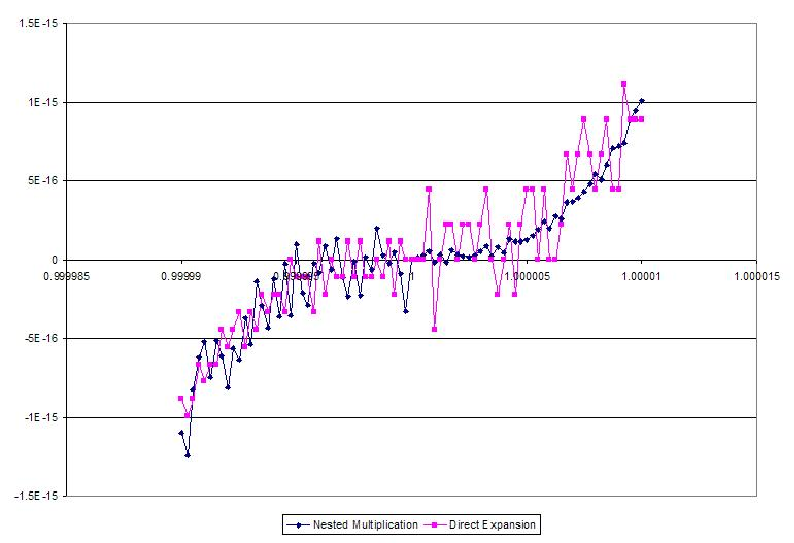
\includegraphics[width=4in]{cubicpoly.png}\\
  \caption{Close-up Look at Resulting Values of Two Evaluation Methods for $y=x^3-3x^2+3x-1$}\label{f-polyeval}
\end{figure}
